\chapter{8PSK and Higher-Order PSK}
\label{ch:8psk}

\begin{nontechnical}
\textbf{8PSK is like using 8 different hand gestures instead of 4}---you can send 50\% more data, but the gestures are closer together, making them easier to confuse!

\textbf{The progression:}
\begin{itemize}
\item \textbf{BPSK:} 2 positions (up/down) = 1 bit/symbol
\item \textbf{QPSK:} 4 positions (4 corners) = 2 bits/symbol
\item \textbf{8PSK:} 8 positions (8 directions) = 3 bits/symbol
\item \textbf{16PSK:} 16 positions = 4 bits/symbol
\end{itemize}

\textbf{Think of it like a compass:} North (000), Northeast (001), East (011), Southeast (110), South (100), Southwest (101), West (010), Northwest (010).

\textbf{The trade-off:} More positions = faster data rate (8PSK is 1.5$\times$ faster than QPSK), but positions are closer together, making them easier to confuse in noise. You need a stronger signal (higher SNR) for reliable detection.

\textbf{Real-world use:} DVB-S2 satellite TV uses 8PSK for HD channels. Satellite bandwidth is expensive, so 50\% more data in the same bandwidth means more channels. Trade-off: you need a bigger dish for 8PSK versus QPSK.

\textbf{Why not go higher?} Beyond 8PSK, positions become too close. Even tiny noise causes errors. QAM (which varies both amplitude and phase) is more efficient---this is why WiFi uses QAM, not 16PSK or 32PSK.
\end{nontechnical}

\section{Overview}

\textbf{8-Phase-Shift Keying (8PSK)} encodes data using 8 equally-spaced phase states around the unit circle, transmitting 3 bits per symbol. This provides a 50\% increase in spectral efficiency compared to QPSK, at the cost of increased SNR requirements.

\begin{keyconcept}
8PSK achieves \textbf{3 bits/symbol} ($\sim$2.2~bps/Hz with $\alpha = 0.35$ pulse shaping), providing \textbf{1.5$\times$ the throughput} of QPSK. However, it requires approximately \textbf{3.5~dB higher $E_b/N_0$} for the same bit error rate due to reduced symbol spacing.
\end{keyconcept}

Higher-order PSK schemes (M-PSK) generalize this concept: $M$ phase states transmit $\log_2(M)$ bits per symbol. However, as $M$ increases beyond 8, phase noise sensitivity and reduced symbol spacing make QAM (Quadrature Amplitude Modulation) more practical.

\textbf{Primary applications:}
\begin{itemize}
\item \textbf{Satellite communications:} DVB-S2 standard for digital television
\item \textbf{Military SATCOM:} MILSTAR and other secure links
\item \textbf{Microwave backhaul:} Point-to-point cellular backhaul
\item \textbf{Deep-space communications:} High-rate science data return
\end{itemize}

\section{Mathematical Description}

\subsection{Time-Domain Signal}

The 8PSK modulated waveform for symbol $m$ is expressed as:
\begin{equation}
s_m(t) = A\cos(2\pi f_c t + \phi_m), \quad 0 \leq t \leq T_s
\end{equation}
where:
\begin{itemize}
\item $A$ = carrier amplitude
\item $f_c$ = carrier frequency (Hz)
\item $T_s$ = symbol period (seconds)
\item $\phi_m$ = phase for symbol $m \in \{0, 1, \ldots, 7\}$
\end{itemize}

\textbf{Phase encoding:} The 8 phase states are equally spaced around the unit circle:
\begin{equation}
\phi_m = \frac{2\pi m}{8} = \frac{\pi m}{4}, \quad m = 0, 1, \ldots, 7
\end{equation}

This gives phase values of: $0°$, $45°$, $90°$, $135°$, $180°$, $225°$, $270°$, $315°$.

\subsection{Complex Baseband Representation}

The complex baseband representation of the $m$-th symbol is:
\begin{equation}
s_m = A e^{j\phi_m} = A e^{j\pi m/4}
\end{equation}

\textbf{In-phase and quadrature components:}
\begin{equation}
I_m = A\cos(\phi_m) = A\cos\left(\frac{\pi m}{4}\right)
\end{equation}
\begin{equation}
Q_m = A\sin(\phi_m) = A\sin\left(\frac{\pi m}{4}\right)
\end{equation}

The transmitted RF signal can be expressed as:
\begin{equation}
s_{\mathrm{RF}}(t) = I_m\cos(2\pi f_c t) - Q_m\sin(2\pi f_c t)
\end{equation}

\subsection{Constellation Diagram}

The 8PSK constellation consists of 8 points equally distributed on a circle of radius $A$:

\begin{center}
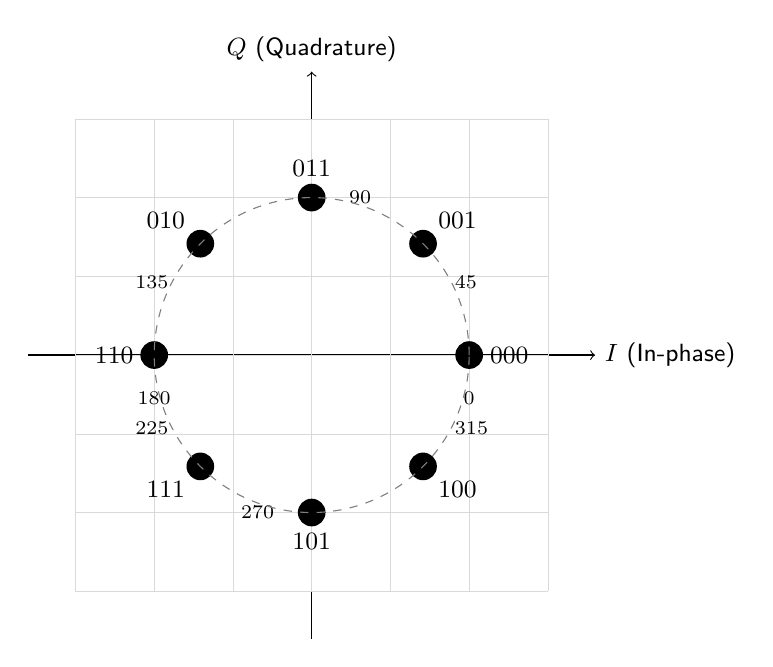
\begin{tikzpicture}[scale=2]
% Axes
\draw[->] (-1.8,0) -- (1.8,0) node[right] {\sffamily\small $I$ (In-phase)};
\draw[->] (0,-1.8) -- (0,1.8) node[above] {\sffamily\small $Q$ (Quadrature)};

% Grid
\draw[very thin,gray!30] (-1.5,-1.5) grid[step=0.5] (1.5,1.5);

% Constellation points with Gray coding
\fill[black] (1,0) circle (2.5pt);
\node[right=4pt,font=\small] at (1,0) {000};
\node[below=10pt,font=\scriptsize] at (1,0) {$0°$};

\fill[black] ({cos(45)},{sin(45)}) circle (2.5pt);
\node[above right=2pt,font=\small] at ({cos(45)},{sin(45)}) {001};
\node[below right=8pt,font=\scriptsize] at ({cos(45)},{sin(45)}) {$45°$};

\fill[black] (0,1) circle (2.5pt);
\node[above=4pt,font=\small] at (0,1) {011};
\node[right=10pt,font=\scriptsize] at (0,1) {$90°$};

\fill[black] ({cos(135)},{sin(135)}) circle (2.5pt);
\node[above left=2pt,font=\small] at ({cos(135)},{sin(135)}) {010};
\node[below left=8pt,font=\scriptsize] at ({cos(135)},{sin(135)}) {$135°$};

\fill[black] (-1,0) circle (2.5pt);
\node[left=4pt,font=\small] at (-1,0) {110};
\node[below=10pt,font=\scriptsize] at (-1,0) {$180°$};

\fill[black] ({cos(225)},{sin(225)}) circle (2.5pt);
\node[below left=2pt,font=\small] at ({cos(225)},{sin(225)}) {111};
\node[above left=8pt,font=\scriptsize] at ({cos(225)},{sin(225)}) {$225°$};

\fill[black] (0,-1) circle (2.5pt);
\node[below=4pt,font=\small] at (0,-1) {101};
\node[left=10pt,font=\scriptsize] at (0,-1) {$270°$};

\fill[black] ({cos(315)},{sin(315)}) circle (2.5pt);
\node[below right=2pt,font=\small] at ({cos(315)},{sin(315)}) {100};
\node[above right=8pt,font=\scriptsize] at ({cos(315)},{sin(315)}) {$315°$};

% Circle
\draw[dashed,gray] (0,0) circle (1);
\end{tikzpicture}
\end{center}

\textbf{Gray coding:} Adjacent symbols differ by only one bit, minimizing bit errors when symbol errors occur. The mapping shown above uses Gray coding to optimize performance.

\begin{center}
\begin{tabular}{@{}ccccc@{}}
\toprule
Symbol & Bits (Gray) & Phase & $I$ & $Q$ \\
\midrule
0 & 000 & $0°$ & $+1.000$ & $0.000$ \\
1 & 001 & $45°$ & $+0.707$ & $+0.707$ \\
2 & 011 & $90°$ & $0.000$ & $+1.000$ \\
3 & 010 & $135°$ & $-0.707$ & $+0.707$ \\
4 & 110 & $180°$ & $-1.000$ & $0.000$ \\
5 & 111 & $225°$ & $-0.707$ & $-0.707$ \\
6 & 101 & $270°$ & $0.000$ & $-1.000$ \\
7 & 100 & $315°$ & $+0.707$ & $-0.707$ \\
\bottomrule
\end{tabular}
\end{center}

Note: I and Q values normalized for $A = 1$.

\section{Signal Properties}

\subsection{Constant Envelope}

A key property of 8PSK is that all symbols have the same amplitude:
\begin{equation}
|s_m| = A, \quad \forall m \in \{0, 1, \ldots, 7\}
\end{equation}

This constant envelope property has important practical benefits:
\begin{itemize}
\item \textbf{Power amplifier efficiency:} Amplifiers can operate at saturation (Class C) without distortion
\item \textbf{Peak-to-Average Power Ratio (PAPR):} 0~dB (ideal constant)
\item \textbf{Nonlinear channel tolerance:} No amplitude information to preserve
\end{itemize}

\begin{warningbox}
While 8PSK has a constant envelope theoretically, \textbf{pulse shaping filters} (e.g., raised-cosine) introduce envelope variations in practice. Typical PAPR with $\alpha = 0.35$ pulse shaping is 3--4~dB, requiring power amplifier backoff to avoid nonlinear distortion.
\end{warningbox}

\subsection{Symbol and Bit Energy}

The energy per symbol is:
\begin{equation}
E_s = \int_0^{T_s} |s_m(t)|^2\,dt = A^2 T_s
\end{equation}

For normalized symbol period $T_s = 1$:
\begin{equation}
E_s = A^2
\end{equation}

Since each symbol carries 3 bits, the energy per bit is:
\begin{equation}
E_b = \frac{E_s}{\log_2(8)} = \frac{E_s}{3} = \frac{A^2}{3}
\end{equation}

\subsection{Minimum Distance}

The Euclidean distance between adjacent constellation points is critical for noise immunity. For 8PSK, adjacent symbols are separated by $45°$:
\begin{equation}
d_{\min} = 2A\sin\left(\frac{\pi}{8}\right) = 2A \times 0.383 = 0.765A
\end{equation}

\textbf{Comparison with QPSK:} For equal symbol energy ($E_s = A^2$):
\begin{itemize}
\item \textbf{QPSK:} $d_{\min} = \sqrt{2}A = 1.414A$
\item \textbf{8PSK:} $d_{\min} = 0.765A$
\item \textbf{Ratio:} 8PSK minimum distance is $1.414/0.765 = 1.85$ times smaller
\end{itemize}

This reduced spacing translates to approximately \textbf{5.3~dB worse performance} for 8PSK compared to QPSK at equal symbol energy, or \textbf{3.5~dB worse} when compared at equal bit energy.

\section{Modulation and Demodulation}

\subsection{Transmitter (Modulator)}

The 8PSK modulator uses the standard IQ modulation architecture:

\begin{center}
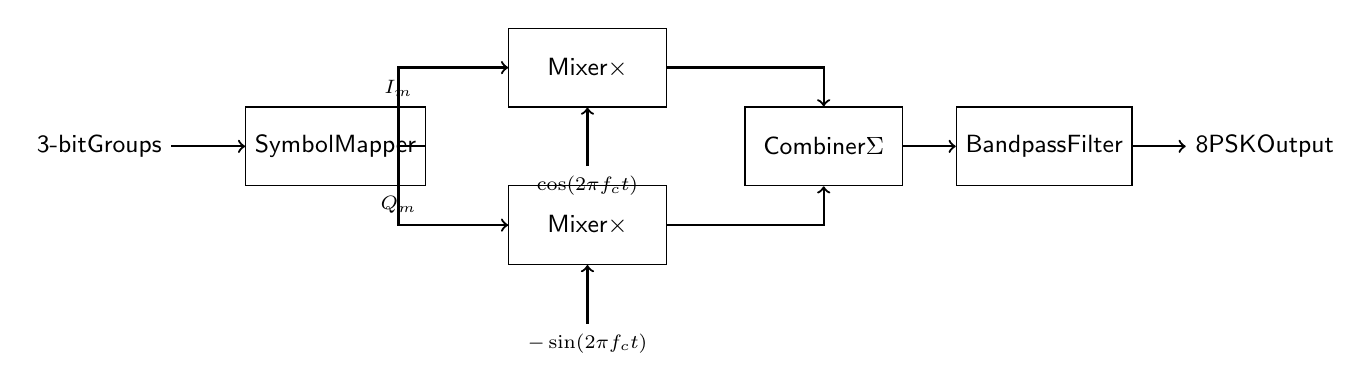
\begin{tikzpicture}[
  block/.style={rectangle, draw, minimum width=2cm, minimum height=1cm, font=\sffamily\small},
  node distance=2cm,
  font=\small
]
\node (input) {\sffamily 3-bit\\Groups};
\node[block, right of=input, node distance=3cm] (mapper) {Symbol\\Mapper};
\node[block, right of=mapper, node distance=3.2cm, yshift=1cm] (imult) {Mixer\\$\times$};
\node[block, right of=mapper, node distance=3.2cm, yshift=-1cm] (qmult) {Mixer\\$\times$};
\node[block, right of=imult, node distance=3cm, yshift=-1cm] (sum) {Combiner\\$\Sigma$};
\node[block, right of=sum, node distance=2.8cm] (bpf) {Bandpass\\Filter};
\node[right of=bpf, node distance=2.8cm] (output) {\sffamily 8PSK\\Output};

\node[below of=imult, node distance=1.5cm, font=\scriptsize] (cos) {$\cos(2\pi f_c t)$};
\node[below of=qmult, node distance=1.5cm, font=\scriptsize] (sin) {$-\sin(2\pi f_c t)$};

\draw[->,thick] (input) -- (mapper);
\draw[->,thick] (mapper) -- ++(0.8,0) |- node[near start,above,font=\scriptsize] {$I_m$} (imult);
\draw[->,thick] (mapper) -- ++(0.8,0) |- node[near start,below,font=\scriptsize] {$Q_m$} (qmult);
\draw[->,thick] (cos) -- (imult);
\draw[->,thick] (sin) -- (qmult);
\draw[->,thick] (imult) -| (sum);
\draw[->,thick] (qmult) -| (sum);
\draw[->,thick] (sum) -- (bpf);
\draw[->,thick] (bpf) -- (output);
\end{tikzpicture}
\end{center}

\textbf{Modulation process:}
\begin{enumerate}
\item \textbf{Symbol mapping:} Map 3-bit groups to I/Q values
\begin{equation}
I_m = A\cos(\phi_m), \quad Q_m = A\sin(\phi_m)
\end{equation}

\item \textbf{IQ modulation:} Mix with carrier quadrature components
\begin{equation}
s_{\mathrm{RF}}(t) = I_m\cos(2\pi f_c t) - Q_m\sin(2\pi f_c t)
\end{equation}

\item \textbf{Pulse shaping:} Apply raised-cosine filter to:
\begin{itemize}
\item Limit occupied bandwidth
\item Control intersymbol interference (ISI)
\item Meet spectral mask requirements
\end{itemize}
\end{enumerate}

\subsection{Receiver (Coherent Demodulator)}

\begin{center}
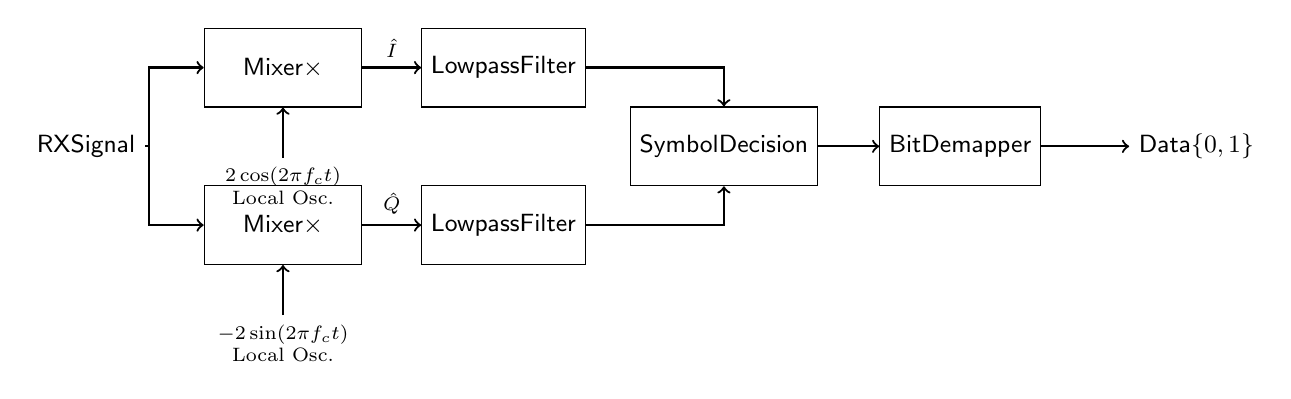
\begin{tikzpicture}[
  block/.style={rectangle, draw, minimum width=2cm, minimum height=1cm, font=\sffamily\small},
  node distance=2cm,
  font=\small
]
\node (input) {\sffamily RX\\Signal};
\node[block, right of=input, node distance=2.5cm, yshift=1cm] (imult) {Mixer\\$\times$};
\node[block, right of=input, node distance=2.5cm, yshift=-1cm] (qmult) {Mixer\\$\times$};
\node[block, right of=imult, node distance=2.8cm] (ilpf) {Lowpass\\Filter};
\node[block, right of=qmult, node distance=2.8cm] (qlpf) {Lowpass\\Filter};
\node[block, right of=ilpf, node distance=2.8cm, yshift=-1cm] (decision) {Symbol\\Decision};
\node[block, right of=decision, node distance=3cm] (demapper) {Bit\\Demapper};
\node[right of=demapper, node distance=3cm] (output) {\sffamily Data\\$\{0,1\}$};

\node[below of=imult, node distance=1.5cm, font=\scriptsize, align=center] (lo1) {$2\cos(2\pi f_c t)$\\Local Osc.};
\node[below of=qmult, node distance=1.5cm, font=\scriptsize, align=center] (lo2) {$-2\sin(2\pi f_c t)$\\Local Osc.};

\draw[->,thick] (input) -- ++(0.8,0) |- (imult);
\draw[->,thick] (input) -- ++(0.8,0) |- (qmult);
\draw[->,thick] (lo1) -- (imult);
\draw[->,thick] (lo2) -- (qmult);
\draw[->,thick] (imult) -- node[above,font=\scriptsize] {$\hat{I}$} (ilpf);
\draw[->,thick] (qmult) -- node[above,font=\scriptsize] {$\hat{Q}$} (qlpf);
\draw[->,thick] (ilpf) -| (decision);
\draw[->,thick] (qlpf) -| (decision);
\draw[->,thick] (decision) -- (demapper);
\draw[->,thick] (demapper) -- (output);
\end{tikzpicture}
\end{center}

\textbf{Demodulation process:}

\begin{enumerate}
\item \textbf{IQ demodulation:} Mix with local oscillator to recover baseband
\begin{equation}
\hat{I} = \int_0^{T_s} r(t) \cdot 2\cos(2\pi f_c t)\,dt
\end{equation}
\begin{equation}
\hat{Q} = -\int_0^{T_s} r(t) \cdot 2\sin(2\pi f_c t)\,dt
\end{equation}

\item \textbf{Phase calculation:}
\begin{equation}
\hat{\phi} = \arctan\left(\frac{\hat{Q}}{\hat{I}}\right)
\end{equation}

\item \textbf{Symbol decision:} Determine closest constellation point. The decision regions are 8 wedges, each $45°$ wide, centered on constellation points:
\begin{equation}
\hat{m} = \left\lfloor \frac{\hat{\phi} + \pi/8}{2\pi/8} \right\rfloor \bmod 8
\end{equation}

\item \textbf{Bit demapping:} Convert symbol index to 3-bit word using Gray code
\end{enumerate}

\begin{warningbox}
\textbf{Phase synchronization is critical.} The local oscillator must be precisely synchronized with the transmitter carrier. A phase offset $\phi_e$ rotates the entire constellation, potentially causing all symbols to be decoded incorrectly. Carrier recovery techniques (Costas loop, decision-directed) are essential.
\end{warningbox}

\subsection{Differential 8PSK (D8PSK)}

Differential encoding provides an alternative that avoids carrier phase ambiguity:

\textbf{Encoding:} Information is encoded in phase transitions rather than absolute phase:
\begin{equation}
\phi_k = \phi_{k-1} + \Delta\phi_k \bmod 2\pi
\end{equation}
where $\Delta\phi_k \in \{0°, 45°, 90°, \ldots, 315°\}$ encodes 3 bits of information.

\textbf{Demodulation:} Compute the phase difference between consecutive symbols:
\begin{equation}
\Delta\hat{\phi}_k = \hat{\phi}_k - \hat{\phi}_{k-1}
\end{equation}

\textbf{Trade-offs:}
\begin{itemize}
\item[\checkmark] \textbf{No carrier phase recovery:} Only frequency synchronization required
\item[\checkmark] \textbf{Simpler receiver:} Eliminates complex carrier tracking loops
\item[\texttimes] \textbf{Performance penalty:} Approximately 3~dB worse than coherent detection
\item[\texttimes] \textbf{Error propagation:} Single detection error affects two consecutive symbols
\end{itemize}

\section{Bit Error Rate (BER) Performance}

\subsection{Symbol Error Rate}

For coherent 8PSK in an additive white Gaussian noise (AWGN) channel, the approximate symbol error rate at high SNR is:
\begin{equation}
P_s \approx 2Q\left(2\sin\left(\frac{\pi}{8}\right)\sqrt{\frac{E_s}{N_0}}\right) = 2Q\left(0.765\sqrt{\frac{E_s}{N_0}}\right)
\end{equation}
where:
\begin{itemize}
\item $E_s$ = energy per symbol (joules)
\item $N_0$ = noise power spectral density (W/Hz)
\item $Q(x) = \frac{1}{\sqrt{2\pi}}\int_x^\infty e^{-t^2/2}\,dt$ is the Gaussian Q-function
\end{itemize}

This approximation assumes errors only occur to adjacent symbols, which is accurate at moderate to high SNR.

\subsection{Bit Error Rate}

With Gray coding, most symbol errors result in single-bit errors. The bit error rate is approximately:
\begin{equation}
\mathrm{BER} \approx \frac{P_s}{\log_2(8)} = \frac{P_s}{3}
\end{equation}

Expressing in terms of $E_b/N_0$ (where $E_b = E_s/3$):
\begin{equation}
\mathrm{BER} \approx \frac{2}{3}Q\left(0.765\sqrt{\frac{3E_b}{N_0}}\right) = \frac{2}{3}Q\left(1.325\sqrt{\frac{E_b}{N_0}}\right)
\end{equation}

\subsection{Required $E_b/N_0$ for Target BER}

For a target BER of $10^{-6}$ (typical for digital communications):

\begin{center}
\begin{tabular}{@{}lcc@{}}
\toprule
Modulation & Required $E_b/N_0$ & Penalty vs QPSK \\
\midrule
BPSK & 10.5~dB & -- \\
QPSK & 10.5~dB & 0~dB (baseline) \\
\textbf{8PSK} & \textbf{14.0~dB} & \textbf{+3.5~dB} \\
16-PSK & 18.0~dB & +7.5~dB \\
32-PSK & 22.0~dB & +11.5~dB \\
\bottomrule
\end{tabular}
\end{center}

\begin{keyconcept}
\textbf{Performance-Efficiency Trade-off:} 8PSK provides 50\% higher spectral efficiency than QPSK (3 vs 2 bits/symbol), but requires 3.5~dB more power for the same BER. This trade-off is fundamental: tighter constellation packing requires higher SNR for reliable detection.
\end{keyconcept}

\subsection{BER Performance Comparison}

The following table shows BER versus $E_b/N_0$ for various PSK modulations:

\begin{center}
\begin{tabular}{@{}ccccc@{}}
\toprule
$E_b/N_0$ (dB) & BPSK & QPSK & 8PSK & 16-PSK \\
\midrule
6~dB & $1.9 \times 10^{-3}$ & $1.9 \times 10^{-3}$ & $4.0 \times 10^{-2}$ & $1.5 \times 10^{-1}$ \\
8~dB & $5.6 \times 10^{-5}$ & $5.6 \times 10^{-5}$ & $8.0 \times 10^{-3}$ & $8.0 \times 10^{-2}$ \\
10~dB & $3.9 \times 10^{-6}$ & $3.9 \times 10^{-6}$ & $7.0 \times 10^{-4}$ & $3.0 \times 10^{-2}$ \\
12~dB & $7.8 \times 10^{-8}$ & $7.8 \times 10^{-8}$ & $4.0 \times 10^{-5}$ & $8.0 \times 10^{-3}$ \\
14~dB & $7.7 \times 10^{-10}$ & $7.7 \times 10^{-10}$ & $1.0 \times 10^{-6}$ & $7.0 \times 10^{-4}$ \\
\bottomrule
\end{tabular}
\end{center}

\textbf{Key observation:} Higher-order PSK requires significantly more SNR to achieve the same BER. The performance penalty increases as constellation density increases.

\section{Bandwidth Efficiency}

The symbol rate for M-PSK is related to the bit rate by:
\begin{equation}
R_s = \frac{R_b}{\log_2(M)}
\end{equation}

For 8PSK: $R_s = R_b/3$ (one symbol carries 3 bits).

With raised-cosine pulse shaping (roll-off factor $\alpha$), the occupied bandwidth is:
\begin{equation}
B = (1 + \alpha)R_s = (1 + \alpha)\frac{R_b}{\log_2(M)} \quad \text{(Hz)}
\end{equation}

The spectral efficiency is:
\begin{equation}
\eta = \frac{R_b}{B} = \frac{\log_2(M)}{1 + \alpha} \quad \text{(bps/Hz)}
\end{equation}

\subsection{Comparison of PSK Schemes}

For $\alpha = 0.35$ (typical value):

\begin{center}
\begin{tabular}{@{}lccc@{}}
\toprule
Modulation & Bits/Symbol & Spectral Efficiency & Required $E_b/N_0$ \\
& & (bps/Hz, $\alpha=0.35$) & (BER $= 10^{-6}$) \\
\midrule
BPSK & 1 & 0.74 & 10.5~dB \\
QPSK & 2 & 1.48 & 10.5~dB \\
\textbf{8PSK} & \textbf{3} & \textbf{2.22} & \textbf{14.0~dB} \\
16-PSK & 4 & 2.96 & 18.0~dB \\
32-PSK & 5 & 3.70 & 22.0~dB \\
\bottomrule
\end{tabular}
\end{center}

\textbf{Fundamental trade-off:} Higher spectral efficiency requires higher SNR. Each doubling of $M$ beyond QPSK adds approximately 3.5--4~dB to the required $E_b/N_0$.

\begin{calloutbox}{Example: 8PSK at 1~Mbps}
\begin{itemize}
\item Data rate: $R_b = 1$~Mbps
\item Symbol rate: $R_s = 1/3 = 333.3$~ksps
\item Roll-off factor: $\alpha = 0.35$
\item Required bandwidth: $B = 1.35 \times 333.3 = 450$~kHz
\item Spectral efficiency: $\eta = 1/0.45 = 2.22$~bps/Hz
\end{itemize}

Compare to QPSK at same data rate:
\begin{itemize}
\item Symbol rate: $R_s = 500$~ksps
\item Required bandwidth: $B = 1.35 \times 500 = 675$~kHz
\item \textbf{Bandwidth savings:} $675 - 450 = 225$~kHz (33\% reduction)
\end{itemize}
\end{calloutbox}

\section{Higher-Order PSK}

\subsection{16-PSK}

16-PSK extends the concept to 16 equally-spaced phase states:

\begin{itemize}
\item \textbf{Phase spacing:} $22.5°$ ($\pi/8$ radians)
\item \textbf{Bits per symbol:} 4
\item \textbf{Minimum distance:} $d_{\min} = 2A\sin(\pi/16) = 0.39A$
\item \textbf{Performance:} Requires $\sim$18~dB $E_b/N_0$ for BER $= 10^{-6}$ (4~dB worse than 8PSK)
\end{itemize}

\textbf{Challenge:} Very sensitive to phase noise due to small angular separation between symbols. Typical oscillator phase noise can cause significant performance degradation.

\subsection{32-PSK and Beyond}

\begin{itemize}
\item \textbf{32-PSK:} $11.25°$ spacing, 5 bits/symbol
\item \textbf{64-PSK:} $5.625°$ spacing, 6 bits/symbol
\end{itemize}

\textbf{Practical limitations:} For $M > 16$, PSK becomes impractical:
\begin{itemize}
\item \textbf{Phase noise sensitivity:} Small angular spacing makes the system extremely sensitive to oscillator instabilities
\item \textbf{Poor SNR efficiency:} Diminishing returns in spectral efficiency versus required $E_b/N_0$
\item \textbf{QAM superiority:} Quadrature Amplitude Modulation (QAM) provides better performance by varying both amplitude and phase
\end{itemize}

\begin{warningbox}
\textbf{Why PSK stops at 8-16 states:} Beyond 8PSK, the phase noise requirements become so stringent that QAM (which uses both amplitude and phase) provides better performance for the same spectral efficiency. This is why modern systems (WiFi, LTE, 5G) use QAM, not high-order PSK.
\end{warningbox}

\section{Comparison with Other Modulations}

\subsection{8PSK vs 16-QAM}

8PSK and 16-QAM achieve similar spectral efficiency ($\sim$2.2~bps/Hz with $\alpha = 0.35$):

\begin{center}
\begin{tabular}{@{}lccl@{}}
\toprule
Parameter & 8PSK & 16-QAM & Winner \\
\midrule
Bits/symbol & 3 & 4 & QAM \\
Spectral efficiency & 2.22~bps/Hz & 2.96~bps/Hz & QAM \\
$E_b/N_0$ (BER $10^{-6}$) & 14.0~dB & 14.5~dB & 8PSK \\
PAPR (ideal) & 0~dB & 2.6~dB & 8PSK \\
PA efficiency & High & Moderate & 8PSK \\
Phase noise tolerance & Moderate & Good & QAM \\
\bottomrule
\end{tabular}
\end{center}

\textbf{Key trade-offs:}
\begin{itemize}
\item \textbf{8PSK advantage:} Constant envelope enables saturated PA operation (higher DC-to-RF efficiency)
\item \textbf{16-QAM advantage:} Better spectral efficiency and more flexibility for adaptive coding
\end{itemize}

\section{Phase Noise Sensitivity}

Oscillator phase noise $\phi_n(t)$ rotates the received constellation:
\begin{equation}
r_m(t) = Ae^{j(\phi_m + \phi_n(t))} + n(t)
\end{equation}

Phase errors cause two effects:
\begin{itemize}
\item \textbf{Rotation:} All symbols rotate by a common offset (correctable with carrier tracking)
\item \textbf{Spreading:} Random jitter blurs the constellation (not correctable)
\end{itemize}

\subsection{Phase Noise Requirements}

The angular spacing between symbols determines phase noise sensitivity:

\begin{center}
\begin{tabular}{@{}lcc@{}}
\toprule
Modulation & Angular Spacing & Relative Sensitivity \\
\midrule
QPSK & $90°$ & Robust \\
8PSK & $45°$ & Moderate \\
16-PSK & $22.5°$ & Sensitive \\
32-PSK & $11.25°$ & Very sensitive \\
\bottomrule
\end{tabular}
\end{center}

\textbf{Rule of thumb:} RMS phase noise should be $< 1/10$ of angular spacing.

\begin{calloutbox}{Example: 8PSK Phase Noise Budget}
For 8PSK with $45°$ spacing:
\begin{itemize}
\item \textbf{Target phase noise:} $< 4.5°$ RMS
\item \textbf{Integrated phase noise:} $\sim$-25~dBc (tight specification)
\item \textbf{Impact:} Requires high-quality oscillators (crystal or temperature-compensated)
\end{itemize}

Compare to QPSK:
\begin{itemize}
\item \textbf{Target phase noise:} $< 9°$ RMS (2$\times$ more tolerant)
\item \textbf{Integrated phase noise:} $\sim$-19~dBc (6~dB more relaxed)
\end{itemize}
\end{calloutbox}

\section{Practical Applications}

\subsection{DVB-S2 (Digital Video Broadcasting - Satellite)}

The DVB-S2 standard uses 8PSK for high-throughput satellite television:

\textbf{Adaptive Coding and Modulation (ACM):}
\begin{itemize}
\item \textbf{Rain fade conditions:} QPSK with rate-1/2 coding (effective: 1~bps/Hz)
\item \textbf{Clear sky:} 8PSK with rate-3/4 coding (effective: 2.25~bps/Hz)
\item \textbf{Throughput gain:} 2.25$\times$ higher data rate when SNR permits
\end{itemize}

\begin{calloutbox}{DVB-S2 Example}
\textbf{Transponder:} 36~MHz bandwidth, Ku-band (12~GHz)

\textbf{Clear weather (high SNR):}
\begin{itemize}
\item Modulation: 8PSK, code rate 3/4
\item Symbol rate: 30~Msps
\item Data rate: $30 \times 3 \times 0.75 = 67.5$~Mbps
\item Can carry $\sim$15 HD channels
\end{itemize}

\textbf{Rain fade (low SNR):}
\begin{itemize}
\item Modulation: QPSK, code rate 1/2
\item Symbol rate: 30~Msps
\item Data rate: $30 \times 2 \times 0.5 = 30$~Mbps
\item Reduced to $\sim$7 HD channels, but maintains reliability
\end{itemize}
\end{calloutbox}

\subsection{Military SATCOM (MILSTAR)}

The MILSTAR military satellite system uses differential 8PSK (D8PSK):
\begin{itemize}
\item \textbf{Anti-jam capability:} Combined with spread spectrum
\item \textbf{Low probability of intercept (LPI):} Differential encoding avoids pilot tones
\item \textbf{Robustness:} Works without precise carrier phase tracking
\end{itemize}

\subsection{Microwave Backhaul}

Point-to-point cellular backhaul links use adaptive modulation:
\begin{itemize}
\item \textbf{Clear weather:} 256-QAM (8 bits/symbol) for maximum throughput
\item \textbf{Rain fade:} Step down to 8PSK, then QPSK as conditions worsen
\item \textbf{Typical bands:} 6--11~GHz, 18~GHz, 23~GHz
\item \textbf{Channel widths:} 28~MHz, 56~MHz standard
\end{itemize}

\subsection{Deep-Space Communications}

NASA and ESA primarily use BPSK/QPSK for maximum link margin, but 8PSK is emerging:
\begin{itemize}
\item \textbf{Mars orbiters:} 8PSK at Ka-band (32~GHz) for science data return
\item \textbf{Trade-off:} 1.5$\times$ data rate versus 3.5~dB link margin loss
\item \textbf{Use case:} High-resolution imagery when spacecraft is close to Earth
\end{itemize}

\section{Implementation Challenges}

\subsection{Carrier Phase Recovery}

8PSK exhibits 8-fold phase ambiguity (every $45°$), requiring robust carrier recovery:

\textbf{Pilot-aided synchronization:}
\begin{enumerate}
\item Insert known pilot symbols periodically
\item Estimate phase offset from pilot correlation
\item Correct data symbols using estimated phase
\end{enumerate}

\textbf{Blind synchronization:}
\begin{itemize}
\item \textbf{8th-power loop:} Raise signal to 8th power to remove modulation, lock to resulting tone
\item \textbf{Decision-directed:} Use decoded symbols to track phase after initial acquisition
\item \textbf{Costas loop:} Phase-locked loop adapted for 8PSK
\end{itemize}

\subsection{Timing Recovery}

Accurate symbol clock is essential. Timing jitter causes:
\begin{itemize}
\item Sampling offset $\rightarrow$ intersymbol interference (ISI)
\item Phase rotation within symbol period
\item Increased BER
\end{itemize}

\textbf{Early-late gate detector:}
\begin{enumerate}
\item Sample at early, on-time, and late positions
\item Compute correlation between early and late samples
\item Adjust clock phase to minimize timing error
\end{enumerate}

\subsection{Power Amplifier Nonlinearity}

While 8PSK has a constant envelope theoretically, pulse shaping introduces amplitude variation:
\begin{itemize}
\item \textbf{Raised-cosine filter:} Creates 3--4~dB PAPR
\item \textbf{PA backoff required:} Reduces DC-to-RF efficiency
\item \textbf{Trade-off:} Spectral containment versus PA efficiency
\end{itemize}

\textbf{Mitigation techniques:}
\begin{itemize}
\item \textbf{Constant-envelope pulse shaping:} MSK, GMSK (eliminates overshoot)
\item \textbf{Digital predistortion:} Pre-distort signal to compensate for PA nonlinearity
\item \textbf{Analog linearization:} Feedforward or feedback amplifier designs
\end{itemize}

\subsection{Frequency Offset Tolerance}

Carrier frequency offset $\Delta f$ causes constellation rotation:
\begin{equation}
r(t) = s(t)e^{j2\pi\Delta f t}
\end{equation}

\textbf{Rule of thumb:} Tolerable frequency offset is $|\Delta f| < 0.01 \times R_s$

\textbf{Example:} 8PSK at 1~Msps
\begin{itemize}
\item Tolerable offset: $< 10$~kHz
\item At $f_c = 1$~GHz: oscillator stability must be $< 10$~ppm
\end{itemize}

\section{Worked Example: 8PSK Link Budget}

\textbf{Scenario:} Geostationary satellite downlink using 8PSK

\subsection*{Given Parameters}

\begin{tabular}{@{}ll@{}}
TX power & $P_t = 20$~W = 43~dBm \\
TX antenna gain & $G_t = 28$~dBi (satellite dish) \\
Distance & $d = 38{,}000$~km (GEO altitude) \\
Frequency & $f_c = 12$~GHz (Ku-band) \\
RX antenna gain & $G_r = 36$~dBi (0.6~m dish) \\
System noise temp & $T_s = 200$~K \\
Bandwidth & $B = 500$~kHz \\
Target BER & $10^{-6}$ \\
Roll-off factor & $\alpha = 0.35$ \\
\end{tabular}

\subsection*{Step 1: Free-Space Path Loss}

\begin{equation}
\mathrm{FSPL}[\mathrm{dB}] = 20\log_{10}(d_{\mathrm{km}}) + 20\log_{10}(f_{\mathrm{MHz}}) + 32.45
\end{equation}
\begin{equation}
\mathrm{FSPL} = 20\log_{10}(38{,}000) + 20\log_{10}(12{,}000) + 32.45 = 205.9~\mathrm{dB}
\end{equation}

\subsection*{Step 2: Received Signal Power}

\begin{equation}
P_r = P_t + G_t + G_r - \mathrm{FSPL}
\end{equation}
\begin{equation}
P_r = 43 + 28 + 36 - 205.9 = -98.9~\mathrm{dBm}
\end{equation}

\subsection*{Step 3: Noise Power}

\begin{equation}
N = kT_sB = (1.38 \times 10^{-23})(200)(500 \times 10^3) = 1.38 \times 10^{-15}~\mathrm{W}
\end{equation}
\begin{equation}
N = 10\log_{10}(1.38 \times 10^{-15}/10^{-3}) = -118.6~\mathrm{dBm}
\end{equation}

\subsection*{Step 4: Carrier-to-Noise Ratio}

\begin{equation}
\mathrm{C/N} = P_r - N = -98.9 - (-118.6) = 19.7~\mathrm{dB}
\end{equation}

\subsection*{Step 5: Data Rate and Symbol Rate}

For 8PSK with $\alpha = 0.35$:
\begin{equation}
R_s = \frac{B}{1 + \alpha} = \frac{500{,}000}{1.35} = 370.4~\mathrm{ksps}
\end{equation}
\begin{equation}
R_b = 3 \times R_s = 3 \times 370.4 = 1.111~\mathrm{Mbps}
\end{equation}

\subsection*{Step 6: $E_b/N_0$ Calculation}

\begin{equation}
\frac{E_b}{N_0} = \mathrm{C/N} + 10\log_{10}\left(\frac{B}{R_b}\right)
\end{equation}
\begin{equation}
\frac{E_b}{N_0} = 19.7 + 10\log_{10}\left(\frac{500{,}000}{1{,}111{,}000}\right) = 19.7 - 3.5 = 16.2~\mathrm{dB}
\end{equation}

\subsection*{Step 7: Link Margin}

\begin{itemize}
\item \textbf{Required $E_b/N_0$ for BER $= 10^{-6}$:} 14.0~dB (8PSK coherent)
\item \textbf{Available $E_b/N_0$:} 16.2~dB
\item \textbf{Link margin:} $16.2 - 14.0 = 2.2$~dB
\end{itemize}

\begin{calloutbox}[colback=black!8!white,colframe=black]{Link Budget Summary}
\textbf{Result: Link closes with 2.2~dB margin}

This tight margin is typical for bandwidth-efficient satellite systems:
\begin{itemize}
\item \textbf{Rain fade:} 2--5~dB typical at Ku-band (exceeds margin)
\item \textbf{Solution:} Adaptive modulation---switch to QPSK during rain
\item \textbf{Clear sky:} Use 8PSK for 1.5$\times$ throughput (1.11~Mbps vs 740~kbps)
\item \textbf{Implementation losses:} $\sim$1--2~dB must be considered in real design
\end{itemize}

\textbf{Conclusion:} 8PSK maximizes throughput in good conditions, but adaptive switching to QPSK ensures reliability during fades.
\end{calloutbox}



\section{Advantages and Disadvantages}

\subsection*{Advantages}

\begin{enumerate}
\item \textbf{Higher spectral efficiency:} 3 bits/symbol provides 50\% more throughput than QPSK in the same bandwidth
\item \textbf{Constant envelope:} Compatible with saturated power amplifiers (Class C), maximizing DC-to-RF efficiency
\item \textbf{Mature technology:} Well-established in satellite and microwave link standards (DVB-S2, etc.)
\item \textbf{Good for bandwidth-limited systems:} When spectrum is expensive or scarce, 8PSK maximizes throughput
\end{enumerate}

\subsection*{Disadvantages}

\begin{enumerate}
\item \textbf{Higher SNR requirement:} Requires 3.5~dB more $E_b/N_0$ than QPSK for the same BER
\item \textbf{Phase noise sensitivity:} $45°$ symbol spacing requires oscillator stability ($< 4.5°$ RMS phase noise)
\item \textbf{Carrier recovery complexity:} 8-fold phase ambiguity necessitates robust synchronization
\item \textbf{Pulse shaping impact:} Raised-cosine filters create 3--4~dB PAPR, reducing PA efficiency benefits
\item \textbf{Limited scaling:} Beyond 8PSK, QAM provides better performance for higher data rates
\end{enumerate}

\section{Summary}

\begin{center}
\begin{tabular}{@{}ll@{}}
\toprule
\textbf{Parameter} & \textbf{Value/Description} \\
\midrule
Bits per symbol & 3 \\
Constellation points & 8 (equally spaced on circle) \\
Phase spacing & $45°$ ($\pi/4$ radians) \\
Spectral efficiency & $\sim$2.2~bps/Hz ($\alpha = 0.35$) \\
BER @ 14~dB $E_b/N_0$ & $1.0 \times 10^{-6}$ \\
Penalty vs QPSK & +3.5~dB $E_b/N_0$ \\
Advantage vs QPSK & +50\% throughput (33\% bandwidth savings) \\
PAPR (ideal) & 0~dB (constant envelope) \\
PAPR (with pulse shaping) & 3--4~dB \\
Carrier recovery & Critical (8-fold ambiguity) \\
Gray coding benefit & $\sim$2$\times$ BER improvement \\
Primary applications & DVB-S2 satellite, microwave backhaul \\
\bottomrule
\end{tabular}
\end{center}

\begin{keyconcept}
\textbf{8PSK Fundamental Trade-off:} 8PSK offers 50\% higher spectral efficiency than QPSK (3 vs 2 bits/symbol) at the cost of 3.5~dB higher power requirement. This makes it ideal for bandwidth-limited systems with adequate SNR, such as satellite communications and fixed microwave links.
\end{keyconcept}

\section{Further Reading}

\begin{itemize}
\item \textbf{Chapter~\ref{ch:bpsk}:} Binary Phase-Shift Keying (BPSK)---foundation of PSK
\item \textbf{QPSK Modulation:} Lower-order PSK with 2 bits/symbol
\item \textbf{Constellation Diagrams:} Visual representation techniques for digital modulation
\item \textbf{Bit Error Rate Analysis:} Performance metrics and measurements
\item \textbf{Carrier Recovery Techniques:} Phase synchronization for coherent detection
\item \textbf{QAM Modulation:} Alternative approach combining amplitude and phase
\item \textbf{Adaptive Modulation and Coding:} Dynamic selection based on channel conditions
\item \textbf{Forward Error Correction:} Coding techniques to improve BER performance
\end{itemize}
